\documentclass{standalone}

\usepackage{pgfplots,tikz,amsmath}
\begin{document}
                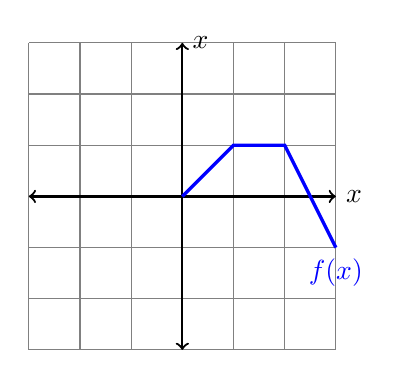
\begin{tikzpicture}[scale=0.65]
                    \draw[color=gray] (-3,-3) grid (3,3);
                    \draw[thick, black, <->] (-3,0) -- (3,0) node[anchor=west]{$x$};
                    \draw[thick, black, <->] (0,-3) -- (0,3) node[anchor=west]{$x$};
                    \draw[very thick, blue] (0,0) -- (1,1) -- (2,1) -- (3,-1)
                    node[anchor=north]{$f(x)$}; 
                \end{tikzpicture}
                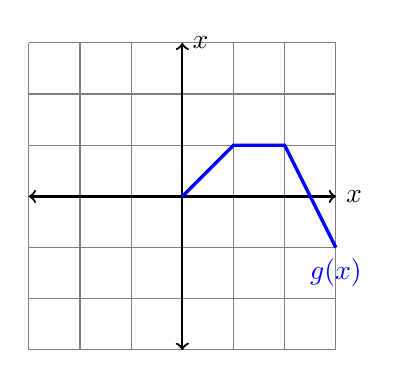
\begin{tikzpicture}[scale=0.65]
                    \draw[color=gray] (-3,-3) grid (3,3);
                    \draw[thick, black, <->] (-3,0) -- (3,0) node[anchor=west]{$x$};
                    \draw[thick, black, <->] (0,-3) -- (0,3) node[anchor=west]{$x$};
                    \draw[very thick, blue] (0,0) -- (1,1) -- (2,1) -- (3,-1)
                    node[anchor=north]{$g(x)$}; 
                \end{tikzpicture}
                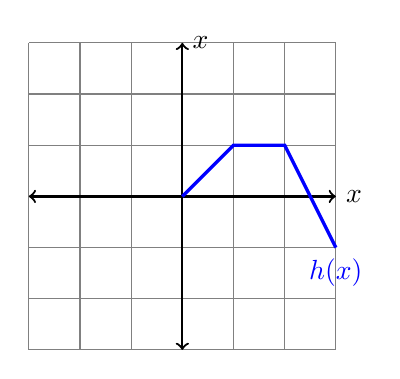
\begin{tikzpicture}[scale=0.65]
                    \draw[color=gray] (-3,-3) grid (3,3);
                    \draw[thick, black, <->] (-3,0) -- (3,0) node[anchor=west]{$x$};
                    \draw[thick, black, <->] (0,-3) -- (0,3) node[anchor=west]{$x$};
                    \draw[very thick, blue] (0,0) -- (1,1) -- (2,1) -- (3,-1)
                    node[anchor=north]{$h(x)$}; 
                \end{tikzpicture}
\end{document}
